\documentclass{article}
\usepackage{tikz}

\begin{document}

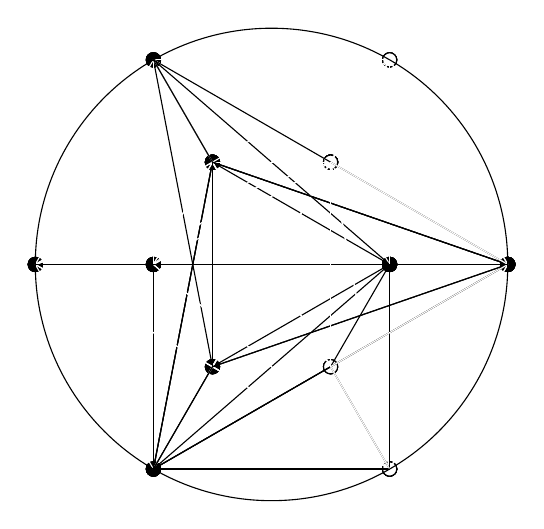
\begin{tikzpicture}[scale=3]
\def\n{6} % set the number of Farey fractions
\def\angle{360/\n} % calculate the angle between each fraction

% Draw the Farey fractions
\foreach \i in {0,...,\n}{
    \foreach \j in {1,...,\i}{
        \pgfmathparse{gcd(\i,\j)==1?"white":"black"} % check if the fraction is in lowest terms
        \edef\colour{\pgfmathresult}
        \draw[fill=\colour] ({\i*\angle}:1) circle (0.03);
        \draw[fill=\colour] ({\j*\angle}:0.5) circle (0.03);
        \draw[fill=\colour] ({(\i-\j)*\angle}:0.5) circle (0.03);
        \draw[fill=\colour] ({(\i+\j)*\angle}:1) circle (0.03);
    }
}

% Draw the edges
\foreach \i in {0,...,\n}{
    \foreach \j in {1,...,\i}{
        \pgfmathparse{gcd(\i,\j)==1?"white":"black"} % check if the fraction is in lowest terms
        \edef\colour{\pgfmathresult}
        \draw[\colour] ({\i*\angle}:1) -- ({\j*\angle}:0.5);
        \draw[\colour] ({\i*\angle}:1) -- ({(\i-\j)*\angle}:0.5);
        \draw[\colour] ({\j*\angle}:0.5) -- ({(\i-\j)*\angle}:0.5);
        \draw[\colour] ({(\i+\j)*\angle}:1) -- ({\j*\angle}:0.5);
        \draw[\colour] ({(\i+\j)*\angle}:1) -- ({\i*\angle}:1);
    }
}

% Draw the disk
\draw (0,0) circle (1);

% Clip the drawing to the interior of the disk
\clip (0,0) circle (1);

\end{tikzpicture}

\end{document}
